% Schematic of the 2-D Yang et al. (2023) setup: square domain HxH, ice
% slab at x in [0.9H, H]. Initial temperature (uniform in y) shown as a
% single red vertical line in the middle of the water block, labeled with
% the water value T_w; the ice value T_i is labeled separately inside the
% thin ice band. Initial salinity (linear ramp in y) shown as a single
% blue inclined line running top (S_top) to bottom (S_bot), on the left
% side of the water block. Standalone TikZ source: compiles on its own
% (pdflatex fig_setup_schematic.tex) and is also includable via \input{}
% or \includegraphics{} in the main article.
\documentclass[tikz,border=4pt]{standalone}
\usepackage{amsmath}
\usepackage{fourier}
\usetikzlibrary{arrows.meta,calc}

\begin{document}
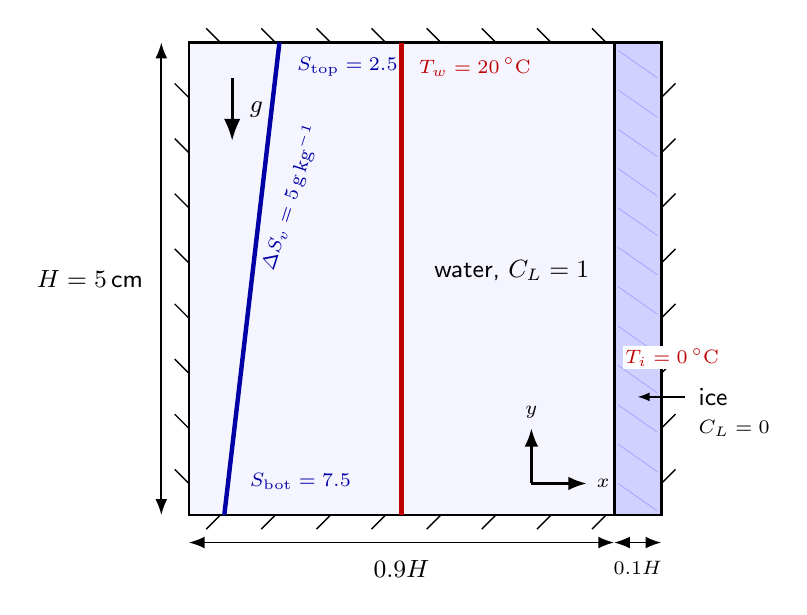
\begin{tikzpicture}[
    >=Latex,
    font=\sffamily\small,
    every node/.style={font=\sffamily\small},
  ]

  % ------------------------------------------------------------------
  % Main domain box: [0,6] x [0,6] represents [0,H] x [0,H]
  % ------------------------------------------------------------------
  \def\Hs{6}          % box side, cm
  \def\xice{5.4}       % 0.9H in box units

  % water (liquid) fill
  \fill[blue!4] (0,0) rectangle (\Hs,\Hs);
  % ice fill
  \fill[blue!18] (\xice,0) rectangle (\Hs,\Hs);
  \foreach \yy in {0.4,0.9,...,5.9} {
    \draw[blue!35, line width=0.3pt] (\xice+0.05,\yy) -- (\Hs-0.05,\yy-0.35);
  }

  % domain border
  \draw[line width=0.9pt] (0,0) rectangle (\Hs,\Hs);

  % no-slip / no-flux tick marks on all four walls -- drawn early so any
  % label placed near a wall (with an opaque white background) is
  % guaranteed to be painted on top of them, not the reverse
  \foreach \xx in {0.4,1.1,...,5.6} {
    \draw[line width=0.5pt] (\xx,0) -- ++(-0.18,-0.18);
    \draw[line width=0.5pt] (\xx,\Hs) -- ++(-0.18,0.18);
  }
  \foreach \yy in {0.4,1.1,...,5.6} {
    \draw[line width=0.5pt] (0,\yy) -- ++(-0.18,0.18);
    \draw[line width=0.5pt] (\Hs,\yy) -- ++(0.18,0.18);
  }

  % ice--water interface (phase boundary), plain black
  \draw[line width=1.1pt] (\xice,0) -- (\xice,\Hs);

  % ------------------------------------------------------------------
  % Temperature: single red vertical line in the middle of the water
  % block (uniform in y); T_w labeled at its top, T_i labeled separately
  % inside the thin ice band
  % ------------------------------------------------------------------
  \def\xT{2.7}
  \draw[red!75!black, line width=1.6pt] (\xT,0) -- (\xT,\Hs);
  \node[anchor=south west, red!75!black, font=\sffamily\scriptsize]
       at (\xT+0.1,\Hs-0.55) {$T_w=20\,^\circ\mathrm{C}$};
  \node[anchor=west, red!75!black, font=\sffamily\scriptsize,
        fill=white, inner sep=1pt]
       at (\xice+0.1,2.0) {$T_i=0\,^\circ\mathrm{C}$};

  % ------------------------------------------------------------------
  % Salinity: inclined blue line on the left side of the water block,
  % drawn top (S_top) to bottom (S_bot) -- stable stratification,
  % denser/saltier water at the bottom
  % ------------------------------------------------------------------
  \draw[blue!65!black, line width=1.6pt] (1.15,\Hs) -- (0.45,0);
  \node[anchor=south west, blue!65!black, font=\sffamily\scriptsize]
       at (1.25,\Hs-0.55) {$S_{\rm top}=2.5$};
  \node[anchor=south west, blue!65!black, font=\sffamily\scriptsize]
       at (0.65,0.2) {$S_{\rm bot}=7.5$};
  \node[anchor=west, blue!65!black, font=\sffamily\scriptsize, rotate=72]
       at (0.95,3.0) {$\Delta S_v=5\,{\rm g\,kg^{-1}}$};

  % region labels
  \node[font=\sffamily\small] at (4.1,3.1) {water, $C_L=1$};
  \node[anchor=west, font=\sffamily\small] at (\Hs+0.35,1.5) {ice};
  \draw[-{Latex[length=1.5mm]}, line width=0.5pt]
       (\Hs+0.3,1.5) .. controls (\Hs+0.0,1.5) .. (\Hs-0.3,1.5);
  \node[anchor=west, font=\sffamily\scriptsize] at (\Hs+0.35,1.1) {$C_L=0$};

  % ------------------------------------------------------------------
  % Axes indicator, inside the box on the right side (bottom-right,
  % just left of the ice band) + gravity arrow, inside the box
  % ------------------------------------------------------------------
  \draw[->, line width=0.8pt] (4.35,0.4) -- (5.05,0.4) node[right, font=\sffamily\scriptsize] {$x$};
  \draw[->, line width=0.8pt] (4.35,0.4) -- (4.35,1.1) node[above, font=\sffamily\scriptsize] {$y$};

  \draw[->, line width=1.1pt] (0.55,5.55) -- (0.55,4.75);
  \node[anchor=west, font=\sffamily\small] at (0.65,5.15) {$g$};

  % ------------------------------------------------------------------
  % Dimension arrows (double-headed): H (left, outside), 0.9H and 0.1H
  % (bottom, outside)
  % ------------------------------------------------------------------
  \draw[<->, line width=0.6pt] (-0.35,0) -- (-0.35,\Hs)
       node[midway,left=3pt,font=\sffamily\small] {$H=5\,\text{cm}$};
  \draw[<->, line width=0.6pt] (0,-0.35) -- (\xice,-0.35)
       node[midway,below=3pt,font=\sffamily\small] {$0.9H$};
  \draw[<->, line width=0.6pt] (\xice,-0.35) -- (\Hs,-0.35)
       node[midway,below=3pt,font=\sffamily\scriptsize] {$0.1H$};

\end{tikzpicture}
\end{document}
